\chapter{Results}

In the following sections, the experiment results are presented and analyzed. Further analysis is provided in the following chapter. The sections are separated based on the experiments that had already described in the previous chapters.

\section{Query modeling}

To answer the first research question about the best query model to improve the performance of our baseline, we conduct the query modeling experiment as it is described in the experimental design chapter. The results of this experiment are presented at the table \ref{table:qmP5}.

\begin{table}[H]
\begin{center}
\caption{System performance using precision at first five results measure (P@5) of title (T), title and description (T+D), all the fields (T+D+A+C) and attribute and categories (A+C) query models using three retrieval strategies (BM25, LM, TfIdf) and two types of ground truth (editorial and click logs).}
\label{table:qmP5}

\begin{tabular}{lccccccc}
\toprule
Query model & \multicolumn{3}{c}{Editorial} & & \multicolumn{3}{c}{Click logs} \\
\midrule
& BM25 & LM & TfIdf &   & BM25 & LM & TfIdf \\
\midrule
T & 0.6560 &  0.5980 & 0.626 &   &         		0.1680 & 0.1660 & 0.1540 \\
T+D & 0.6660 & 0.5880 & 0.6500 &   &    			0.1700 & 0.1680 & \textbf{0.1600} \\
T+D+A+C & \textbf{0.7300} & \textbf{0.6460} & \textbf{0.6860} &   & \textbf{0.1720} & \textbf{0.1700} & 0.1580 \\
A+C & 0.4800 & 0.3400 & 0.4500 &   &     			0.0920 & 0.0900 & 0.0600 \\
\bottomrule
\end{tabular}
\end{center}
\end{table}

The table \ref{table:qmP5} represents the precision at five first results from four different query models. First, we are adding fields to our baseline to see if any improvement occurs. The last query model with only attributes and category is an extra query model to investigate if it consists of enough information to improve the precision of our baseline.

In the results with the editorial evaluation, adding the description to our baseline shows an improvement on precision using BM25 and TfIdf, except LM that shows a minor decrease. Adding the attributes and category gives a boost to all retrieval strategies. However, precision of query model with attributes and category is worse than our baseline's precision.

The results using the click logs evaluation indicate a slight increase in the precision when the description is used in the query models. Also, adding the attributes and category, shows a small increase but not on TfIdf. However, the attributes and category alone in the query model are not performing better than the baseline.

The results verify our initial assumption that adding extra information on the title query model can improve the performance. We can give an initial answer before further analysis to the first research question that using all the fields on the query model indicates the highest precision thus is the best one of the available query models.


\section{Retrieval modeling}

Second research question that we are answering is about the best retrieval method from the three available (Okapi BM25F, TfIdf and LM). In the table \ref{table:qmP5}, we can compare the difference in precision bettween different retrieval methods and same query models. Furthermore, on table \ref{table:rmInc}
 we present the increase in precision using BM25F over LM and the difference in precision using BM25F over TfIdf.

\begin{table}[H]
\begin{center}
\scriptsize
\caption{ Percentage increase on presicion 
\% increase of presision using BM25 instead of LM and increase of presision using BM25 instead of TfIdf. Query models used are title (T), title and description (T+D), all the fields (T+D+A+C) and attribute and categories (A+C) query models two types of ground truth (editorial and click logs).}
\label{table:rmInc}

\begin{tabular}{lccccc}
\toprule
 & \multicolumn{2}{c}{Editorial} & &\multicolumn{2}{c}{Click logs} \\
\midrule
Query model & \% BM25 over LM & \% BM25 over TfIdf &   &  \% BM25 over LM & \% BM25 over TfIdf\\
\midrule
T & 9.7 & 4.8 &   & 1.2 & 9.1 \\
T+D & 13.3 & 2.5 &   & 1.2 & 6.2 \\
T+D+A+C & 13  & 6.4  &   & 1.2 & 8.9 \\
A+C & 41.2 & 6.7 &   &  2.2 & 53.3 \\

\bottomrule
\end{tabular}
\end{center}
\end{table}


 In the results of the table \ref{table:qmP5} with editorial evaluation, LM has the smallest precision in a comparison with the other two. Systems are using BM25F increase the precision of systems using LM at least 13\% using editorial evaluation and at least 1,2\% using click logs evaluation. Incerase on precision on systems using BM25F over the systems using TfIdf is at least 2.5\% using editorial evaluation and 6.2\% using click logs evaluation.
 Furthermore, in results with click logs evaluation in one query model LM and TfIdf have the same precision. However, in attributes and category query models TfIdf has lower precision than LM.


Provided with the previous results, we can verify that Okapi BM25 is the retrieval strategy which performs better than the other two.


 However, is important to mention here that retrieval methods are using smooth parameters that we didn't experimented with them like ...... The assumptions we are making in this section are based on the default parameters and experimenting with them might give different results thus further investigation is needed.


\section{Late data fusion}

Different late data fusion techniques used to answer the third research question about improving the performance of the individual systems using these techniques.

\begin{table}[H]
\begin{center}
\footnotesize
\caption{System performance using precision at first five results measure (P@5) of late data fusion methods (combMAX, combMIN, combSUM, combMNZ, combANZ, WcombSUM, WcomMNZ, WcombWW) and the best individual system using two types of ground truth (editorial and click logs).}
\label{table:ldfP5}

\begin{tabular}{lcr}
\midrule
  & Editorial & Clicks logs\\
 \midrule
 	Best individual & \textbf{0.7300} & 0.1720 \\
	combMAX & 0.5400 & 0.1280\\
	combMIN & 0.0760 & 0.0020 \\
	combSUM & 0.6160 & 0.1720 \\
	combMNZ & 0.6460 & 0.1720 \\
	combANZ & 0.0800 & 0.0020 \\
	WcombSUM & 0.6140 & \textbf{0.1740} \\
	WcombMNZ & 0.6360 & \textbf{0.1740} \\
	WcombWW & 0.6320 & \textbf{0.1740} \\
\bottomrule
\end{tabular}
\end{center}
\end{table}


The table \ref{table:ldfP5} represents all the late fusion methods we use to answer the third research question in a comparison with the individual best system. The most important observation of this table is that none of the fused systems is performing better than the individual one using the editorial evaluation.

On the results with the editorial evaluation, the combMNZ is performing better than the rest of the fused systems. The rest of the fused systems have small differences in the precision except of the combMIN and combANZ that have very low precision.

On the results with click logs evaluation, the weighted fused systems have better precision than the rest. Then, a slight decrease in precision is seen on combMNZ and combMAX and a bigger decrease on combMAX. Same as editorial evaluation, the combANZ and combMIN have the lowest precision.


\section{Diversification}

In this set of experiments we answer the following research questions:

The research questions we aim to answer are the following:
\begin{enumerate}
\item Are the results of diversification affected if only the similarity with the previous displayed classified is taken into account?
\item Are the results of diversification affected if the average similarity of previous displayed docs is taken into account?
\item Are the results of diversification affected if only the similarity with the previous four displayed classifieds is taken into account?
\end{enumerate}

% Overall Accuracy
\begin{figure}[H]
\centering
\begin{minipage}{.5\textwidth}
	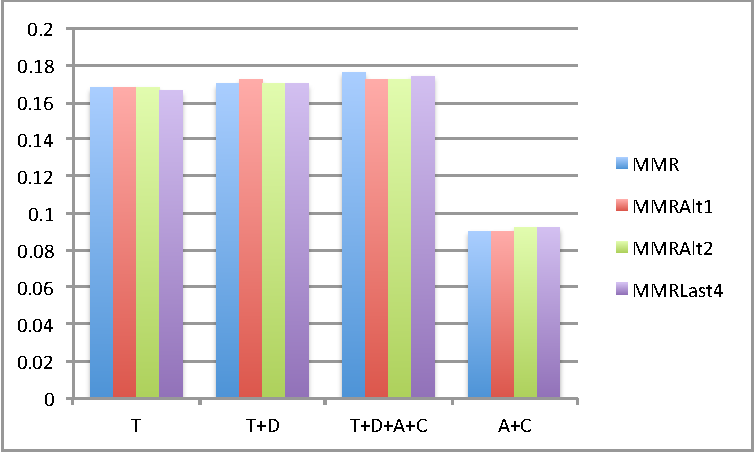
\includegraphics[width=.9\linewidth]{../images/MMRMethodsP@5.pdf}
	\subcaption{Click logs}
	\label{fig:acc-ns}
\end{minipage}%
\begin{minipage}{.5\textwidth}
	\centering
	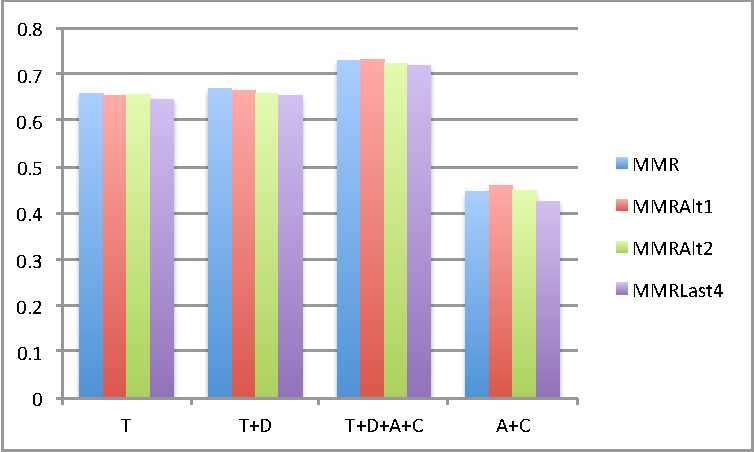
\includegraphics[width=.9\linewidth]{../images/MMRMethodsP@5Relevance.pdf}
	\subcaption{Editorial}
	\label{fig:acc-ns}
\end{minipage}%
\caption{Bar graphs with the system performance (P@5) of diversification methods MMR, MMRAlt1, MMRAlt2, MMRLast4 using title (T), title and description (T+D), all the fields (T+D+A+C) and attribute and categories (A+C) query models and two types of ground truth (editorial and click logs).
}
\end{figure}


In the figure 5.1, the precision at five first results for the diversification methods using four different query models is presented. In both graphs the trends are almost the same thus none of the systems performs better than the others. So, as a first conclusion that can make with regard to the diversification research questions (four, five and six) is that none of which performs better than the MMR method proposed on \cite{CarbonellGoldstein}.


\section{Fused diversified results}

The final research question is weather fusing diversified ranked lists improves the performance of the not diversified systems.

\begin{table}[H]
\begin{center}
\scriptsize
\caption{System performance using precision at first five results measure (P@5) of late data fusion methods (combMAX, combMIN, combSUM, combMNZ, combANZ, WcombSUM, WcombMNZ, WcombWW) of fused system and fused diversified system using two types of ground truth (editorial and click logs). Also, percentage increase from fused diversified results over the fused not diversified (\% IOD) is provided for both ground truths.}
\label{table:ldfMmrP5}

\begin{tabular}{lccccccc}
\toprule
 & \multicolumn{3}{c}{Editorial} & & \multicolumn{3}{c}{Click logs} \\
\midrule
 & Fused diversified & Fused not diversified & \% increase &   & Fused diversified & Fused not diversified & \% increase\\
 \midrule
	combMAX & \textbf{0.7320} & 0.5400 & 35.5\% &   & 0.1700 & 0.1280 & 32.8\\
	combMIN & 0.0800 & 0.0760 & 5.3 &   & 0.0020 & 0.0020 & 0\\
	combSUM & 0.6700 & 0.6160 & 8.8 &   & 0.1720 & 0.1720 & 0 \\
	combMNZ & 0.6700 & 0.6460 & 3.7 &   & 0.1720 & 0.1720 & 0\\
	combANZ & 0.0940 & 0.0800 & 17.5 &   & 0.0040 & 0.0020 & 100\\
	WcombSUM & 0.6620 & 0.6140 & 7.8 &   & 0.1720 & \textbf{0.1740} & -1.15\\
	WcombMNZ & 0.6560 & 0.6360 & 3.1 &   & 0.1720 & \textbf{0.1740} & -1.15\\
	WcombWW & 0.6560 & 0.6320 & 3.8 &   & 0.1720 & \textbf{0.1740} & -1.15\\
\bottomrule
\end{tabular}
\end{center}
\end{table}

The table \ref{table:ldfMmrP5} represents the comparison of the fused diversified systems versus the fused individual systems with both click logs and editorial evaluation to answer this reasearch question.

Using the click logs evaluation, we can see that the precision of combANZ is doubled when we fuse the diversified instead of fuse the not diversified ranked lists. Also, the precision increased by 32.8\% on combMAX fusion of diverified system over the combMAX fusion of not diversified systems. The rest of the fusion methods either they don't have any improvement or they even have decrease  in acomparison of the fusion of diversified systems with the fusion of not diversified.

Using editorial evaluation show us an improvement on the precision when the diversified lists are fused. Also, the biggest difference is in the combMAX which has an increase of 0.19. The smallest increase we have in table \ref{table:ldfMmrP5} is the combANZ which is 0.014. Also, combMAX fusion of diversified ranked lists outperforms even our best individual system (T+D+A+D) using BM25F by 11.6\%. 

Further measurements of data fusion of all the proposed diversification methods can be seen on \ref{table:LdfMmr}, \ref{table:LdfMmralt1}, \ref{table:LdfMmralt2}, \ref{table:LdfMmrAvgLast4}.

In sum, using the editorial evaluation we can verify and answer to the seventh research question that the fused diversified systems perform better than the fused not diversified systems. Using the click log evaluation, we can not give the same answer cause the results in the table don't show any large improvement.


Research questions had already been answered with the results of this chapter. A deeper analysis and assumptions about the reasons we have these results are provided in the next chapter.
